\begin{frame}{Semantic Embedding \& Vector Search}

\begin{columns}[T]
  \begin{column}{0.50\textwidth}
    \textbf{Sentence Embedding with \tech{MiniLM}:}
    \begin{itemize}
      \item \highlight{Model:} \tech{all-MiniLM-L6-v2}
      \item \highlight{Input format:}
        {\scriptsize \textit{"Title: ... Author: ... Description: ..."}}
      \item \highlight{Output:} 384-dimensional vectors
      \item \highlight{Advantage:} Semantic similarity beyond keywords
    \end{itemize}

    \vspace{0.3cm}
    \textbf{Vector Search with \tech{FAISS}:}
    \begin{itemize}
      \item \highlight{Index:} 5,160 book embeddings
      \item \highlight{Search:} L2 distance (exact search)
      \item \highlight{Performance:} $<$ 10ms query time
      \item \highlight{Local:} No external dependencies
    \end{itemize}

	\vspace{0.2cm}
    \textbf{Why \tech{MiniLM} Specifically:}
    \begin{itemize}
        \item Balance of performance vs size
        \item Small enough to run locally in real-time
        \item But powerful enough for semantic understanding
    \end{itemize}

  \end{column}

  \begin{column}{0.45\textwidth}
    \centering
    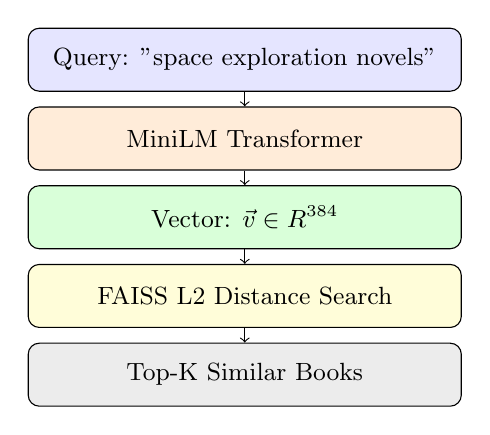
\begin{tikzpicture}[node distance=1.0cm, every node/.style={font=\small}]
        % Embedding process
        \node (input) [draw, rounded corners, minimum width=5.5cm, minimum height=0.8cm, fill=blue!10] 
        {\small Query: "space exploration novels"};

        \node (embed) [below of=input, draw, rounded corners, minimum width=5.5cm, minimum height=0.8cm, fill=orange!15] 
        {\small MiniLM Transformer};

        \node (vector) [below of=embed, draw, rounded corners, minimum width=5.5cm, minimum height=0.8cm, fill=green!15] 
        {\small Vector: $\vec{v} \in \mathbb{R}^{384}$};

        % Search process
        \node (faiss) [below of=vector, draw, rounded corners, minimum width=5.5cm, minimum height=0.8cm, fill=yellow!15] 
        {\small FAISS L2 Distance Search};

        \node (results) [below of=faiss, draw, rounded corners, minimum width=5.5cm, minimum height=0.8cm, fill=gray!15] 
        {\small Top-K Similar Books};

        % Arrows
        \draw[->] (input) -- (embed);
        \draw[->] (embed) -- (vector);
        \draw[->] (vector) -- (faiss);
        \draw[->] (faiss) -- (results);
    \end{tikzpicture}
    
    \vspace{0.2cm}
    \small \textit{End-to-end semantic search in $<$ 200ms}
  \end{column}
\end{columns}

\end{frame}

\note{
	\begin{columns}[T]
    	\begin{column}{0.49\textwidth}
			[TIMING: 1.5 min Embeddings - CORE TECHNICAL SLIDE]
			\begin{itemize}
			  \item "Embeddings convert text to numbers that capture meaning - 384 dimensions means each book becomes a point in 384D space"
			  \item "Books with similar meanings cluster together in this space -Like a map where distance represents semantic similarity"
			\end{itemize}
			
			\vspace{0.1cm}
			[CONCRETE EXAMPLE (use the diagram):]
			\begin{itemize}
			  \item "User types 'space exploration novels' - MiniLM converts this to 384 numbers"
			  \item "FAISS finds books whose embeddings are closest"
			  \item "Might find 'Mars colonization story', 'astronaut memoir' - no exact keyword matches needed!"
			\end{itemize}
			
			\vspace{0.1cm}
			[PERFORMANCE EMPHASIS:]
			\begin{itemize}
			  \item "Sub-200ms total - feels instant to users"
			  \item "Most time in embedding query, search is nearly instant"
			  \item "Scales well - current dataset tiny compared to FAISS capabilities"
			\end{itemize}
			\end{column}
			
			\begin{column}{0.49\textwidth}
			[TECHNICAL DEPTH (if asked):]
			\begin{itemize}
			  \item "Could use cosine similarity but L2 works well for normalized embeddings"
			  \item "FAISS uses optimized algorithms for billion-scale search"
			  \item "IndexFlatL2 = exact search, could use approximate for speed"
			\end{itemize}
			
			\vspace{0.1cm}
			[POTENTIAL QUESTIONS:]
			\begin{itemize}
			  \item \textit{"Why not larger models like BERT?"} → "Size vs performance tradeoff - need to run locally"
			  \item \textit{"How does semantic similarity work?"} → "Model trained to put similar meanings close together in vector space"
			  \item \textit{"What if user query very different from training?"} → "May not work well - limitation of current approach"
			  \item \textit{"Could you use approximate search?"} → "Yes, FAISS has IVF, LSH options for speed vs accuracy tradeoff"
			\end{itemize}
			
			\vspace{0.1cm}
			[TRANSITION:]
			\begin{itemize}
			  \item "Let me show you how this looks in the actual user interface..."
			\end{itemize}
    \end{column}
  \end{columns}
}
